\chapter{Introducción}
\label{chap:introduccion}


\section{Los desechos espaciales}

El comienzo de la era satelital en el a\~no 1957 con la puesta en \'orbita del sat\'elite ruso Sputnik signific\'o la conquista de un nuevo espacio y un cambio de paradigma en lo que respecta a las tecnolog\'ias para las comunicaciones, los estudios de nuestro planeta, el sistema solar, las formas de navegar, de geoposicionarse y el intercambio de informaci\'on. Desde entonces el ambiente espacial cada vez suma m\'as colonos (Fig. \ref{fig:cantidad2014}).\\

Las experiencias de las primeras misiones aportaron mucho conocimiento de este entorno con caracter\'isticas muy distintas a las de la superficie de la Tierra y permitieron ir mejorando las t\'ecnicas y los materiales para que los sat\'elites cumplieran sus objetivos sin mayores inconvenientes.
Sin embargo, un hecho poco predicho o abordado empez\'o a ocupar prioridad en las dos \'ultimas d\'ecadas: los {\it{desechos espaciales}}.\\

{\bf{Definici\'on:}}{\it{ Son Desechos Espaciales todos los objetos construidos por el hombre, incluyendo fragmentos o partes de los mismos, que orbitan la Tierra o reingresan a la atm\'osfera y no son funcionales, es decir, han perdido su capacidad operativa.}} \citep{iadcguide}\\

La disponibilidad del espacio parec\'ia ilimitada, y los primeros a\~nos no se ten\'ian consideraciones respecto a los objetos que all\'i se depositaban, o se desprend\'ian de los cohetes y las misiones. Pero con el correr del tiempo, ciertas regiones del espacio cobraron inter\' es estrat\'egico, y la superpoblaci\'on en dichas zonas no tard\'o en mostrar complicaciones.\\

Los desechos representan hoy el mayor porcentaje de los objetos que orbitan la Tierra y los estudios de su proliferaci\'on, indican que, de no existir planes de acci\'on para subsanar la situaci\'on, el efecto de las colisiones en cascada transformar\'a el ambiente espacial en un lugar inhabitable para cualquier misi\'on.\\

La primera colisi\'on confirmada y claramente registrada entre una misi\'on operativa y un desecho, ocurri\'o el 24 de Julio de 1996, cuando el sat\'elite franc\'es Cerise (95-033B) fue embestido por un fragmento (86-019RF), remanente de la explosi\'on de la \'ultima etapa del cohete Ariane-1 H-10, ocurrida el 13 de noviembre de 1986; nueve meses despu\'es de inyectar en \'orbita al sat\'elite SPOT-1. La reconstrucci\'on de la situaci\'on luego de la colisi\'on, coincide plenamente con una p\'erdida de la actitud del Cerise que fue registrada en los datos hist\'oricos abordo \citep{KlinkradChapter8}.\\

%Este accidente fue un disparador en lo que respecta al estudio de los desechos espaciales y las colisiones. (correcion walkiria)
Las estad\'isticas de la base de datos de Scopus \footnote{https://www.scopus.com/}, indican que las investigaciones respecto a la tem\'atica de desechos espaciales en general muestran un continuo crecimiento (Fig. \ref{fig:scopusSD}). Resultados similares se obtienen respecto de la tem\'atica de colisiones (Fig. \ref{fig:scopusCA}); si bien no se ha podido hacer una vinculaci\'on directa entre sucesos, picos y tendencias, se mencionan algunos eventos que podr\'ian estar relacionados con los resultados. En el a\~no 1988 la \ac{NASA} implementa su sistema para analizar y evitar colisiones en las misiones tripuladas ({\it{Collision Assessment and Collision Avoidance System}}), a continuaci\'on en el a\~no 1990 se lanza el telescopio espacial {\it{Hubble Space Telescope}} y se realiza un congreso de gran trascendencia, el {\it{Orbital Debris Conference: Technical Issues and Future Directions }}. Se observa un pico a partir del a\~no 1998, probablemente vinculado al lanzamiento de la estaci\'on espacial internacional o \ac{ISS}, y luego un notorio crecimiento a partir del a\~no 2007, vinculado a dos sucesos: la destrucci\'on intencional de China de uno de sus sat\'elites en una prueba misil\'istica y la colisi\'on catastr\'ofica accidental entre el sat\'elite ruso KOSMOS 2251, fuera de servicio y el sat\'elite IRIDIUM 33, operativo, de la constelaci\'on de IRIDIUM, en el a\~no 2009.\\

%La misma tendencia puede verse en la tem\'atica de colisiones (Fig. \ref{fig:scopusCA}), destac\'andose el gran escal\'on a partir del a\~no 1993 (colisi\'on del sat\'elite Cerise),



\begin{figure}[!h]
\centering
  \textbf{Publicaciones sobre Desechos Espaciales (Scopus)}\par\medskip
    \fbox{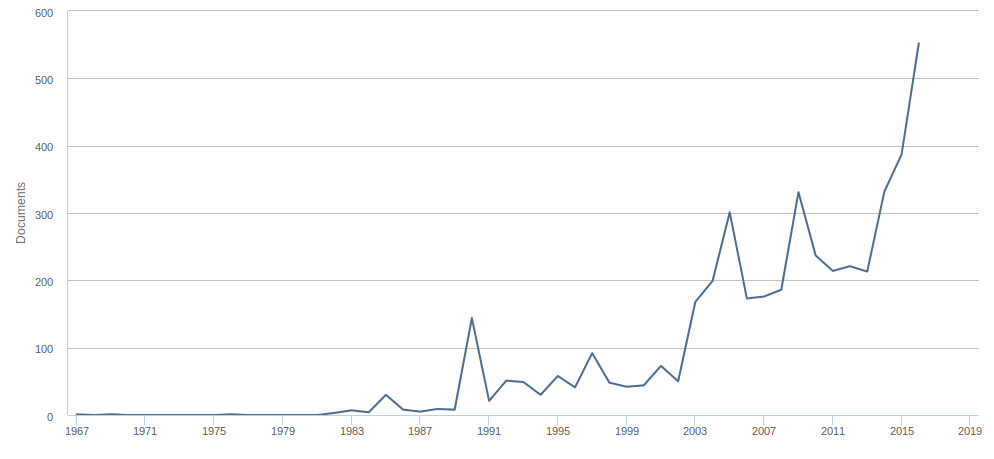
\includegraphics[width=0.8\columnwidth, keepaspectratio]{imagenes/scopusSD}}
    \caption[Desechos Espaciales seg\'un Scopus]{Estad\'istica de las investigaciones realizadas en el \'area de desechos espaciales ({\it{Space Debris}}) de acuerdo a la base de datos de Scopus.}
    \label{fig:scopusSD}
\end{figure}

\begin{figure}[!h]
\centering
   \textbf{Publicaciones sobre Colisiones (Scopus)}\par\medskip
    \fbox{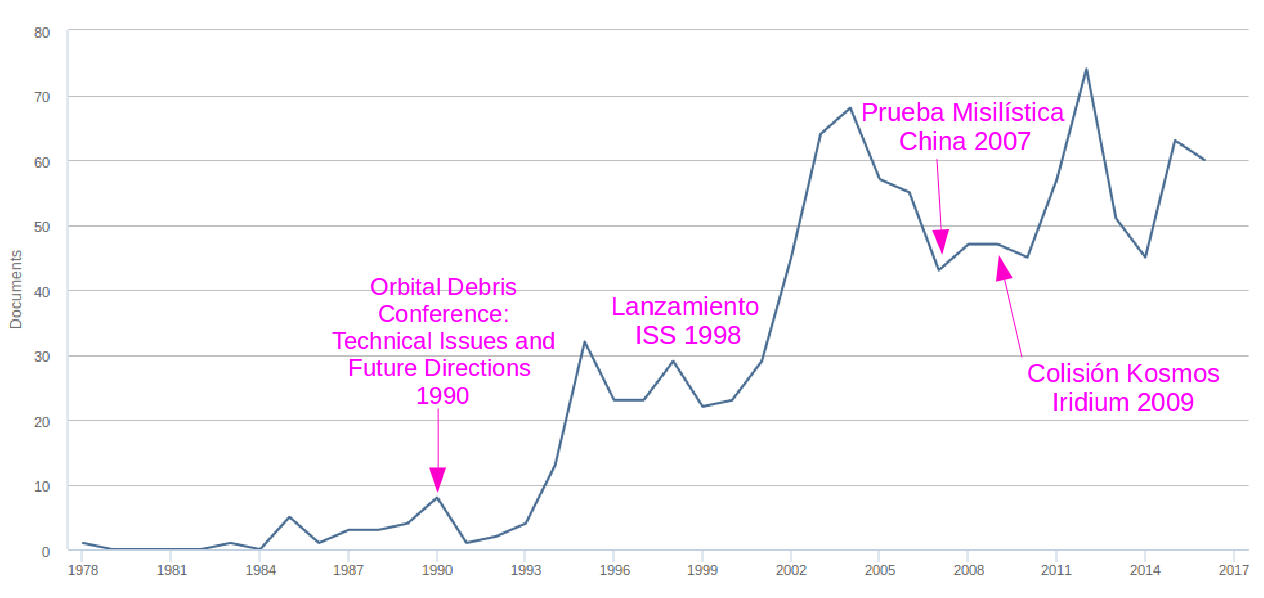
\includegraphics[width=0.7\columnwidth, keepaspectratio]{imagenes/scopusCA}}
    \caption[Riesgos de Colisi\'on seg\'un Scopus]{Estad\'istica de las investigaciones realizadas en el \'area de riesgos de colisi\'on {\it{Collision Avoidance}} de acuerdo a la base de datos de Scopus.}
    \label{fig:scopusCA}
\end{figure} 

\subsection*{Distintos abordajes para el estudio de los desechos espaciales}
Existen distintos estudios respecto a la problem\'atica de los desechos espaciales. La \ac{NASA} propone una clasificaci\'on general seg\'un sean estudios de: modelado, rastreo, protecci\'on, mitigaci\'on, reparaci\'on o reingreso.\\
\begin{itemize}
%\setlength{\itemsep}{0pt}
\item {\bf{Modelado:}} Consiste en el desarrollo y la actualizaci\'on de los modelos orbitales de los desechos, para describir y caracterizar el ambiente actual y la proyecci\'on futura.\\
\item {\bf{Rastreo:}} Mediciones que se hacen con radares y telescopios \'opticos desde tierra, y tambi\'en con telescopios espaciales.\\
\item {\bf{Protecci\'on:}} Estudios hechos en impactos de alta velocidad para el desarrollo de nuevos materiales y dise\~nos que ofrezcan una mayor protecci\'on.\\
\item {\bf{Mitigaci\'on:}} Planifiaci\'on de estrategias para reducir la generaci\'on de nuevos desechos. Generaci\'on de documentaci\'on  de buenas pr\'acticas, est\'andares y promoci\'on de acuerdos internacionales.\\
\item {\bf{Reparaci\'on:}} Dise\~no de misiones con el \'unico objetivo de actuar sobre los desechos a fin de reducir el n\'umero de objetos inactivos en \'orbita.\\
\item {\bf{Reingreso:}} Identificaci\'on de los reingresos no controlados, para hacer an\'alisis sobre las zonas de posibles impactos en Tierra y la planificaci\'on de reingresos controlados.\\
\end{itemize}

Organismos como el Centro Principal de Inteligencia Espacial Ruso, el Departamento de Defensa Norteamericano, la NASA y la \ac{ESA}, han desarrollado tanto modelos de evoluci\'on como de ingenier\'ia, y mantienen cat\'alogos actualizados con las trayectorias de aquellos objetos cuyo tama\~no permite detectarlos con instrumentos de rastreo en Tierra.\\

Los modelos de evoluci\'on muestran la configuraci\'on actual y proyecciones de configuraciones futuras del ambiente espacial incluyendo todos los objetos que orbitan la Tierra.\\

Los modelos de ingenier\'ia se enfocan en distintas pruebas de laboratorio o de misiones espec\'ificas en \'orbita, que analizan la respuesta de los materiales cuando se exponen a impactos con fragmentos de distinto tipo, particularmente en aquellos de tama\~nos muy chicos pero que colisionan a velocidades del orden de diez kil\'ometros por segundo.\\

En este trabajo nos enfocamos en el an\'alisis de las situaciones de riesgo de colisi\'on, dentro del marco de la {\it{mitigaci\'on}}, para las misiones y los desechos que se ubican en las  \ac{LEO}, u \'orbitas bajas.\\

\subsection*{El entorno de los desechos espaciales: presente y futuro}
Seg\'un los informes de la \ac{ESA} \citep{esaSD}, desde 1957 hasta la actualidad, 5250 lanzamientos han poblado el ambiente espacial con casi 23000 objetos de los cuales, s\'olo cerca de 1200 son sat\'elites operativos.\\

El \ac{IADC}, clasifica los desechos seg\'un sean: objetos relacionados a alguna misi\'on, fragmentos, o cohetes y objetos que ya finalizaron su misi\'on (Tabla \ref{tab:desechosIADC}).\\

\begin{table}[!h]
\caption[Clasificaci\'on de Desechos seg\'un la IADC]{Clasificaci\'on de desechos, causas y recomendaciones del IADC}
\resizebox{17.5cm}{!}{
\begin{tabular}[c]{cll}
\hline 
\rowcolor{lightgray}
\bf{Clasificaci\'on}  &    \bf{Causas} & \bf{Recomendaciones del IADC}\\
\hline
\multirow{ 2}{*}{Objetos relacionados a una misi\'on} &   Liberados intencionalmente& Dise\~nos que reduzcan la liberaci\'on de desechos\\
&Liberados sin intenci\'on& Dise\~nos robustos\\
\hline
\multirow{ 4}{*}{Fragmentos}& Destrucci\'on intencional & Evitar destrucciones intencionales.\\
& Fragmentaciones durante las operaciones & Aseguramiento de la misi\'on.\\
& Fragmentaciones ya finalizada la misi\'on & Reducci\'on de estas situaciones en el dise\~no.\\
& \cellcolor{blue!25}{Colisiones en \'orbita} & Planificaci\'on de maniobras evasivas por riesgo\\
&&de colisi\'on. Protecci\'on.\\
\hline
Objetos que ya finalizaron & Maniobras de disposal inadecuadas &Maniobras de reingreso\\
su misi\'on y cohetes && \\
\hline
\end{tabular} }
\label{tab:desechosIADC}
\begin{flushleft}
\small {\it{Nota.}} Adaptado de la gu\'ia de recomendaciones del IADC, \citep{iadcguide}.
\end{flushleft}
\end{table}


De a acuerdo a una publicaci\'on de la NASA, \citep{ODQNum}, hasta el 04 de Abril de 2017, se contabilizaron $18347$ objetos catalogados (Tabla \ref{tab:objpais}). Clasificados seg\'un sean: cargas \'utiles ({\it{payloads}}), cohetes ({\it{rocket bodies}}), desechos de misi\'on ({\it{mission-related bodies}}), desechos an\'omalos ({\it{anomalous debris}}) o desechos de fragmentaci\'on ({\it{breakup debris}}); ver Figura \ref{fig:catxtipo}.\\

\begin{table}
 \caption[Objetos en \'Orbita al 4 de Abril de 2017.]{Objetos en \'Orbita al 4 de Abril de 2017.}
 \begin{tabular}{lccc}
  \hline 
  \rowcolor{lightgray}
  \bf{Pa\'is}  &    \bf{Cargas \'Utiles} & \bf{Cohetes y Desechos} & TOTAL\\
  \hline 
  China & 235 & 3566&3801\\
  Comunidad de Estados Independientes & 1508&4993&6501\\
  Agencia Espacial Europea &74&60&134\\
  Francia & 62&470&532\\
  India & 79 & 113 & 192\\
  Jap\'on & 162 & 94 & 256\\
  Estados Unidos de Am\'erica & 1513 & 4504 & 6017\\
  Otros & 801 & 113 & 914 \\
  \hline
  \rowcolor{lightgray}
  TOTAL & 4434 & 13913 & 18347 \\
  \hline
 \end{tabular}
 \label{tab:objpais}
 \begin{flushleft}
\small {\it{Nota.}}  Adaptado de NASA, \citep{ODQN}.
\end{flushleft}
\end{table}

\begin{figure}[!h]
\centering
    \fbox{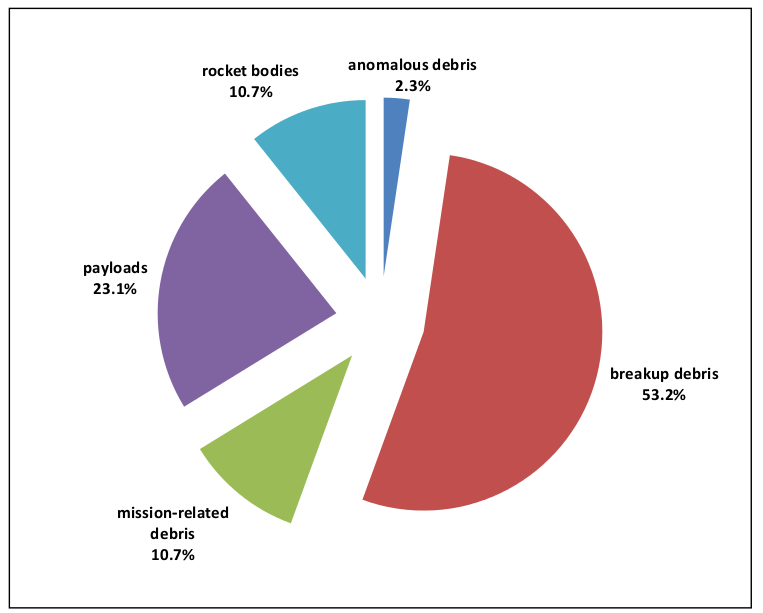
\includegraphics[width=0.7\columnwidth, keepaspectratio]{imagenes/clasificacion2016}}
    \caption[Objetos en \'Orbita seg\'un NASA.]{Porcentaje de Objetos en \'Orbita seg\'un la clasificaci\'on de NASA. Extra\'ido de NASA, \citep{ODQN}.}
    \label{fig:catxtipo}
\end{figure}

Otra clasificaci\'on podr\'ia ser en funci\'on de la distancia a la superficie de la Tierra, ya que la distribuci\'on no es homog\'enea. La relaci\'on entre la densidad de objetos y la altura a la que se encuentran, señala que existen regiones m\'as comprometidas.
Las \'orbitas bajas o \ac{LEO} con un rango de alturas entre los 500 y los 2000 kil\'ometros, son las m\'as superpobladas y contienen casi el 70 \% de todos los objetos catalogados. 
Cabe destacar que en esta regi\'on se ubican las misiones de la serie SAC de la CONAE, las misiones futuras SAOCOM Y SABIAMAR. Ver Figura \ref{fig:Dvsaltura}.\\

\begin{figure}[!h]
  \centering
  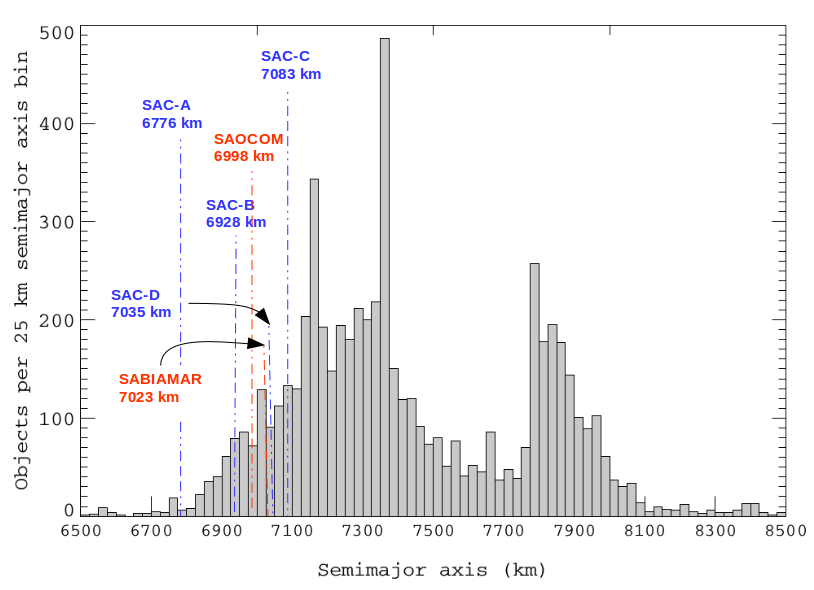
\includegraphics[width=0.9\textwidth]{imagenes/SDvsaltura2011CONAE}
  \caption[Distribuci\'on de objetos en funci\'on del semieje mayor.]{Distribuci\'on de objetos en funci\'on del semieje mayor en la regi\'on LEO. Adapatado de \citep{Klinkrad}. Se agregan en color azul las posiciones de las misiones de CONAE ya puestas en \'orbita (serie SAC) y en color naranja las posiciones de las futuras misiones SAOCOM y SABIAMAR}
  \label{fig:Dvsaltura}
\end{figure}

Si se mira hacia el futuro, las predicciones no son alentadoras. Si bien, los acuerdos internacionales en relaci\'on a acciones para reducir la proliferaci\'on de desechos avanzan y muestran buenos resultados, los proyectos de nuevas misiones tienden a aumentar el n\'umero de objetos, sobre todo en las \'orbitas bajas. Para estas \'orbitas las colisiones pasar\'ian a ser las principales generadoras de desechos.\\

En un reporte t\'ecnico publicado por la NASA \citep{karacalioglu2016impact}, se eval\'uan las nuevas tendencias de la industria satelital y se analiza el futuro panorama del entorno espacial en las \'orbitas bajas, en funci\'on de los lanzamientos planificados y las misiones anunciadas, (Fig. \ref{fig:satxlanz}).\\

En los \'ultimos a\~nos se ha incrementado el n\'umero de agencias o empresas que se dedican al desarrollo espacial. El nuevo paradigma de constelaciones de peque\~nos sat\'elites, sistemas distribuidos o arquitecturas fragmentadas en reemplazo de los grandes y costosos sat\'elites tradicionales, ha permitido la democratizaci\'on del espacio, facilit\'andole el acceso a m\'as agencias y empresas. 
Un claro ejemplo son las constelaciones para comunicaciones anunciadas por OneWeb y SpaceX, que proyectan lanzar del orden de 600 sat\'elites cada una para fines del 2019.

\begin{figure}[!h]
  \centering
  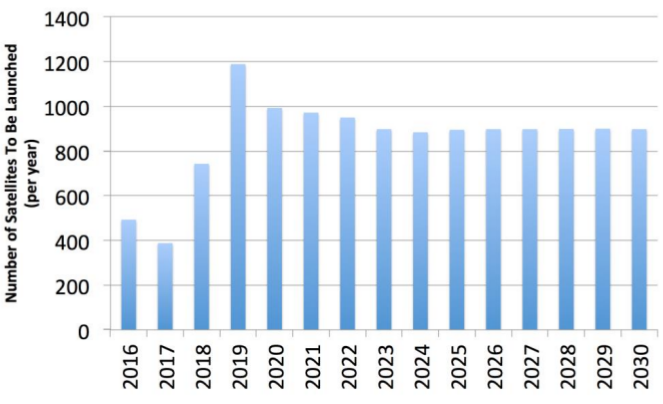
\includegraphics[width=0.7\textwidth]{imagenes/satelxlanz}
  \caption[Proyecci\'on de Sat\'elites 2016-2030]{Proyecci\'on de Sat\'elites 2016-2030. Extra\'ido de \citep{karacalioglu2016impact}}
  \label{fig:satxlanz}
\end{figure}

Estas futuras misiones, no s\'olo generan un aumento en la poblaci\'on espacial durante su vida \'util, sino que, una vez finalizada la misi\'on es importante definir acciones que remuevan esos objetos de la regi\'on de LEO; ya que dependiendo de sus caracter\'isticas, pueden permanecer en \'orbita inactivos por m\'as de 20 a\~nos.\\

A su vez, aunque ya existen modelos experimentales y en desarrollo en lo que respecta a recuperar partes de los lanzadores, cada lanzamiento inyecta en \'orbita no s\'olo los sat\'elites sino tambi\'en las \'ultimas etapas de los cohetes lanzadores, (Fig. \ref{fig:rocketbodies}).\\

\begin{figure}[!h]
  \centering
  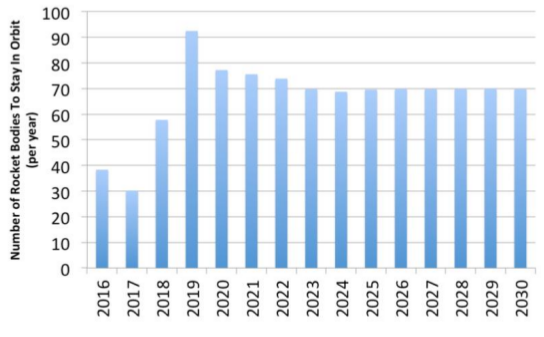
\includegraphics[width=0.7\textwidth]{imagenes/rocketbodies}
  \caption[Fragmentos de Cohetes 2016-2030]{Fragmentos de Cohetes que permanecer\'an en \'orbita en el periodo 2016-2030. Extra\'ido de \cite{karacalioglu2016impact}}
  \label{fig:rocketbodies}
\end{figure}

\section{El riesgo de colisi\'on}

La primera colisi\'on catastr\'ofica que se registra, sucedi\'o en el a\~no 2009, entre el sat\'elite ruso KOSMOS \- 2251 que hab\'ia quedado fuera de servicio y el sat\'elite operativo IRIDUM 33 de la constelaci\'on de IRIDIUM.\\

El evento ocurri\'o a 790 kil\'ometros de altura y gener\'o m\'as de 2500 fragmentos, de los cuales, 500 a\'un permanecen en \'orbita. Este suceso, marc\'o la materializaci\'on de una situaci\'on que se preve\'ia que pod\'ia ocurrir y ofici\'o de catalizador de los estudios vinculados a la predicci\'on, an\'alisis y mitigaci\'on del riesgo de colisi\'on (Fig. \ref{fig:scopusCA}).\\

De los distintos modelos de evoluci\'on y de las descripciones del ambiente espacial a trav\'es de los a\~nos, se distingue claramente, c\'omo aumenta el n\'umero de desechos cuando ocurren colisiones significativas. As\'i puede apreciarse en la Figura. \ref{fig:cantidad2014}, donde la curva magenta, que se\~nala los desechos producidos por fragmentaciones, sube abruptamente a comienzos del a\~no 2007 debido a la destrucci\'on intencional del sat\'elite chino Fengyun, en una prueba misil\'istica, y en 2009 con la colisi\'on entre el IRIDIUM 33 y el KOSMOS que mencion\'abamos m\'as arriba.\\

\begin{figure}[!h]
  \centering
  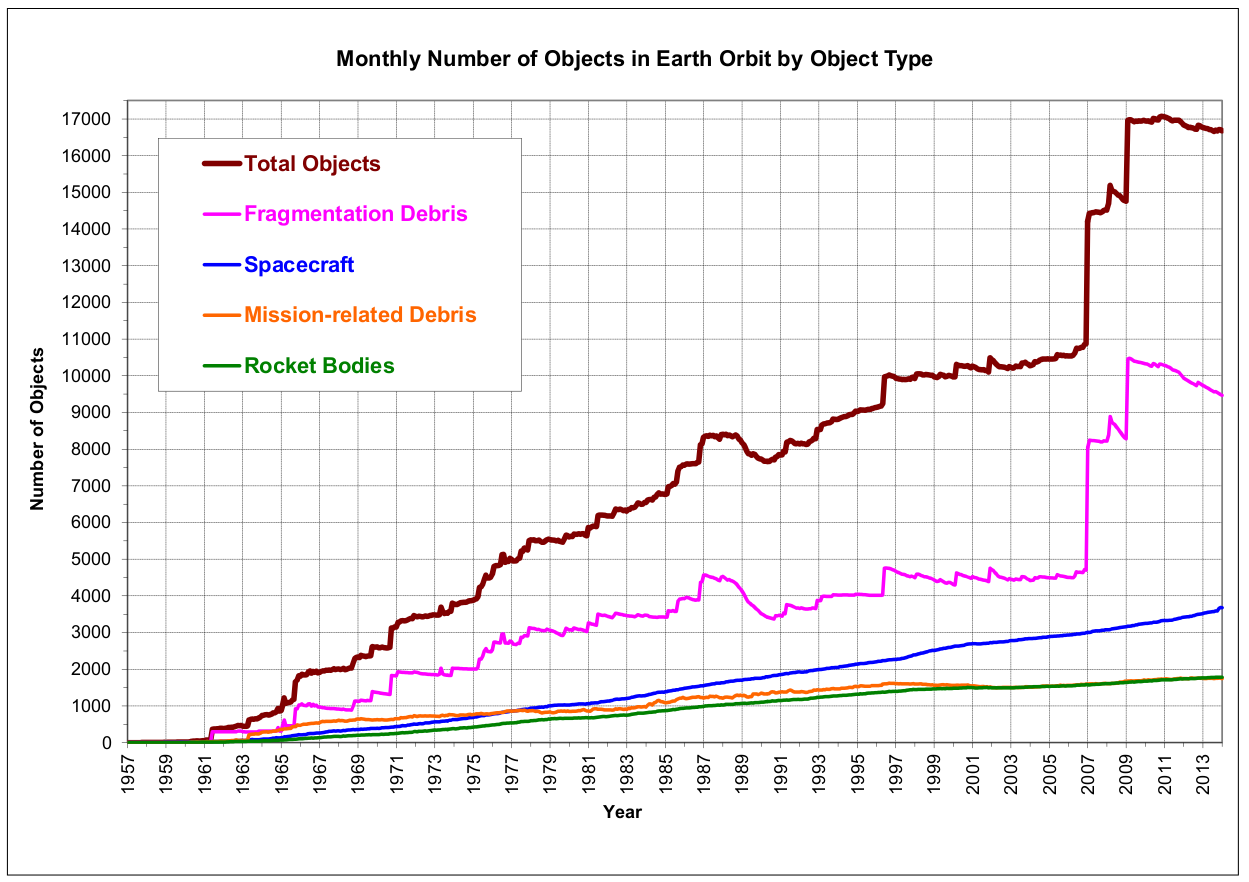
\includegraphics[width=0.8\textwidth]{imagenes/numero2014}
  \caption[Cantidad de Objetos catalogados al 2014]{Cantidad de Objetos catalogados al 2014 - Se distingue el incremento abrupto producto de las fragmentaciones del Fengyun Chino en 2007 y de la colisi\'on entre el IRIDIUM y el Kosmos en 2009.Extra\'ido de \citep{ODQN14}}
  \label{fig:cantidad2014}
\end{figure}

En esta problem\'atica, se produce una retroalimentaci\'on negativa, en donde, a partir del incremento de objetos, en particular en las \'orbitas LEO, aumentan las colisiones, convirti\'endose las mismas, a su vez, en las principales fuentes de generaci\'on de desechos.\\ 

La Figura \ref{fig:causadesechos} muestra que el porcentaje del remanente de desechos producto de rupturas debido a diferentes causas, fue modific\'andose en los \'ultimos a\~nos. Las distintas pol\'iticas de mitigaci\'on en relaci\'on a explosiones intencionales, restos de combustibles, el tratamiento de las bater\'ias y la protecci\'on de los materiales frente a impactos, han reducido el n\'umero de desechos asociados a estas cuestiones y a causas desconocidas; no obstante, los desechos generados por colisiones han aumentado.\\

\begin{figure}[!h]
  \centering
  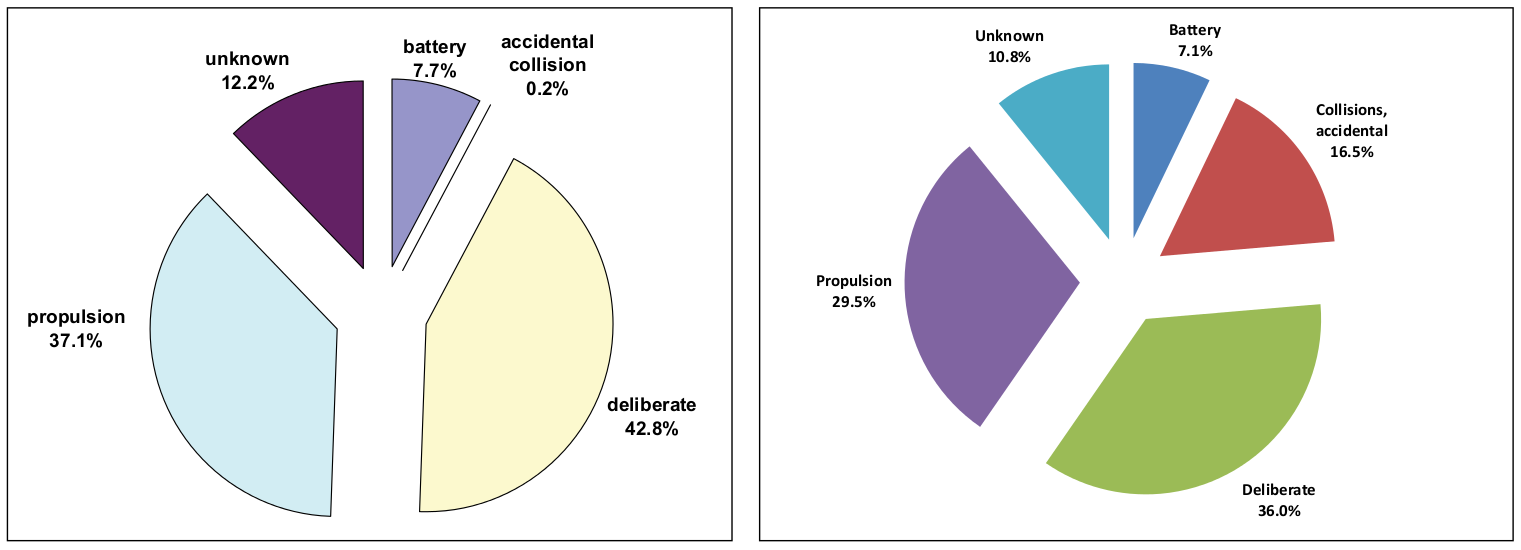
\includegraphics[width=0.8\textwidth]{imagenes/breakupsQNews}
  \caption[Evoluci\'on de las causas de la generaci\'on de Desechos]{Evoluci\'on de las causas de la generaci\'on de Desechos entre 2007 y 2016. Extra\'ido de \citep{ODQNum}}
  \label{fig:causadesechos}
\end{figure}

Conclusiones similares se desprenden del estudio de Karacalioglu \citep{karacalioglu2016impact}, cuyas simulaciones futuras se\~nalan que en los pr\'oximos a\~nos ser\'an las colisiones las que mayor n\'umero de desechos aporten al total de objetos que orbitan la Tierra en las \'orbitas bajas (Fig. \ref{fig:debriscollision}).\\

\begin{figure}[!h]
  \centering
  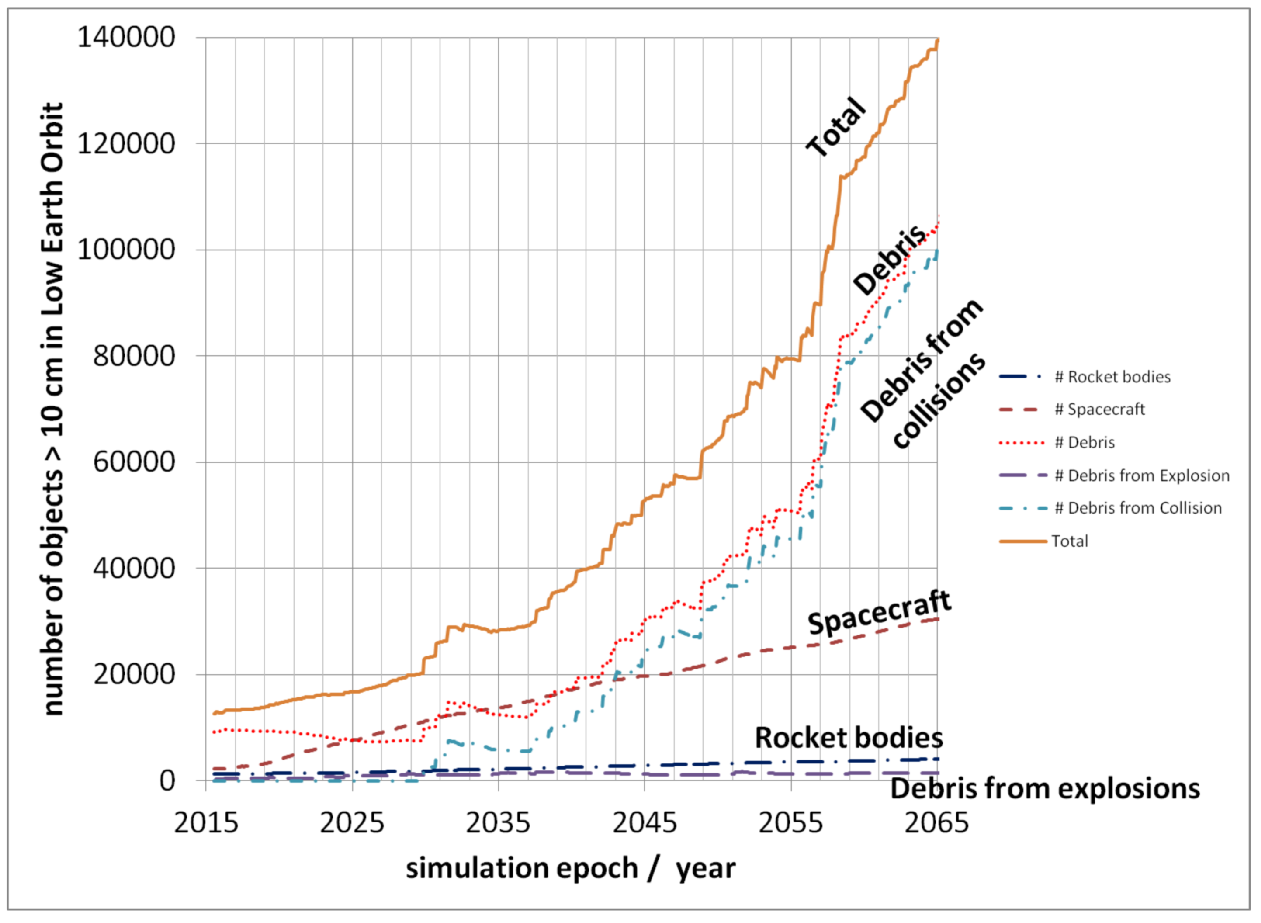
\includegraphics[width=0.7\textwidth]{imagenes/debriscollision}
  \caption[N\'umero de Desechos en las \'orbitas LEO desde 2015 al 2065]{N\'umero de desechos mayores a 10 cm, en las \'orbitas LEO desde 2015 al 2065. La mayor cantidad de desechos en el futuro ser\'an generados producto de las colisiones (curva celeste). Extra\'ido de \citep{karacalioglu2016impact}}
  \label{fig:debriscollision}
\end{figure}

Ya en 1978  estudios hechos por D. Kessler y Cour-Palais,
 \citep{kessler0}, anunciaban el riesgo del efecto en cascada que podr\'ian producir las colisiones, aumentando los desechos en un camino catastr\'ofico sin fin y mostrando que los desechos generados por colisiones superar\'ian los impactos por meteoritos.\\
 
 Por su parte los modelos de ingenier\'ia ofrecen una descripci\'on de los distintos efectos que producen los impactos, dependiendo del tama\~no del desecho. Ver Tabla \ref{tamanioDanio}\\
 
 \begin{table}[h]
 \caption[Da\~no seg\'un el tama\~no del desecho.]{Da\~no producido por el impacto con un desecho en funci\'on del tama\~no del desecho.}
\begin{tabular}[c]{c| l}
\hline
\hline
Tama\~no m\'inimo de la  &    Efecto\\
part\'icula que genera el efecto & \\
\hline
\hline
\multirow{ 7}{*}{100 $\mu$m }& * Da\~no significativo en sensores sensibles.\\
& (Las ventanas del transbordador requieren recambio)\\
& * Corta ataduras, anclajes y cables.\\
& * Penetraci\'on de las multicapas de aislaci\'on (MLI)\\
& * Penetraci\'on de las paredes con grosores de 300 a 500 $\mu$m.\\
& * Penetraci\'on de los tubos de calefacci\'on y radiadores.\\
& * Penetraci\'on de celdas solares.\\
\hline 
\multirow{ 5}{*}{1 mm }& * Cr\'ateres y perforaciones de 2 mm a 1 cm de di\'ametro\\
& dependiendo del tipo del material y el grosor.\\
& * Penetraci\'on de las paredes con grosores de 3-5 mm.\\
& Da\~no del equipamiento detr\'as de las paredes.\\
& *Penetraci\'on de tanques y cables externos.\\
\hline
\multirow{ 3}{*}{1 cm } & * Da\~no estructural y destrucci\'on de alguna parte impactada.\\
& * Penetraci\'on de todas las capas\\ %, incluyendo modulos tripulados\\
& con protecci\'on especial.\\
\hline
\multirow{ 2}{*}{10 cm } & * Destrucci\'on total del sat\'elite o del subsistema impactado.\\
& * Interferencia con observaciones astron\'omicas.\\
\hline
\multirow{ 2}{*}{1m}& * Partes s\'olidas de la plataforma pueden sobrevivir\\
& y reingresar a la atmósfera, incluso alcanzando la superficie.\\
\hline
\end{tabular}
\label{tamanioDanio}
\begin{flushleft}
\small {\it{Nota.}}  Extra\'ido de IADC 08/03, Versi\'on 2.1, Abril 2013
\end{flushleft}
\end{table}

\subsection{El estudio del riesgo de colisi\'on}\label{subsec:estudiocolision}

Para evitar impactos que comprometan significativamente la salud del sat\'elite, la nave debe contar con la capacidad de realizar una maniobra en los casos en los que el objeto de choque tenga un tama\~no considerable, a saber, mayor a los 10 cm de di\'ametro. No obstante, objetos de este tama\~no, pueden ser rastreados y catalogados, lo que permite predecir acercamientos y hacer an\'alisis de las distintas situaciones.\\

A partir del estudio de la situaci\'on orbital de los objetos y los errores involucrados, se estiman ciertos par\'ametros (Ver Sec. \ref{sec:probcol}) que luego son comparados a valores definidos bajo ciertos criterios para concluir si el sat\'elite se encuentra en una situaci\'on de riesgo.\\ 

Un an\'alisis completo del riesgo de colisi\'on abarca, (Fig. \ref{fig:estudiocolision}):

\begin{itemize}
\setlength{\itemsep}{0pt}
\item Identificar las situaciones de encuentro.
\item Analizar la situaci\'on del encuentro.
\item Ejecutar maniobras de mitigaci\'on del riesgo si fuera necesario.
\item Iterar el proceso en forma minuciosa para no ofrecer soluciones moment\'aneas que generen nuevos riesgos de colisi\'on.
\end{itemize}

\subsubsection*{Identificaci\'on de las situaciones de encuentro:}
A partir de los datos generados por las redes de rastreo (Sec.\ref{subsec:redes}), se propagan las trayectorias orbitales y, bajo ciertos criterios definidos previamente, se detectan los acercamientos no deseados.\\
En esta idea subyace la definici\'on de {\it{Encuentro}}.\\

Son pocos los organismos y agencias capaces de realizar este procedimiento, incorporando a sus predicciones todos los objetos catalogados y/o rastreados. En un esquema m\'as simplificado, el inter\'es se enfoca en una misi\'on en particular y se desarrollan filtros, para procesar encuentros analizando una menor cantidad de objetos.\\


\subsubsection*{An\'alisis de la situaci\'on del encuentro: }
El mismo consiste en estudiar el encuentro con mayor profundidad y detalle, sumando informaci\'on m\'as confiable en la determinaci\'on orbital, y calculando par\'ametros estad\'isticos, como la probabilidad de colisi\'on, \ac{PoC}.\\

A medida que se aproxima la fecha en la que se predice el encuentro, se tiene mejor conocimiento de la \'orbita de los objetos involucrados, pero menor tiempo de reacci\'on en la toma de decisiones. Es decir, en el an\'alisis del encuentro se busca un balance entre los tiempos que conlleve el estudio para alcanzar la confiabilidad necesaria, y el margen que se requiere para, por ejemplo, planificar una maniobra. En este \'item en particular se enfoca este trabajo.\\

\subsubsection*{Realizaci\'on de una maniobra:}
Si la situaci\'on lo ameritara, la \'unica manera de evitar una colisi\'on es la {\bf{realizaci\'on de una maniobra}}, conocidas como Maniobras de Mitigaci\'on de Riesgo o \ac{RMM}. No obstante, modificar la trayectoria de un objeto, siempre presupone una evaluaci\'on a priori de que no vaya a producirse una colisi\'on. De manera, que en este punto, se realizan propagaciones con las posiciones estimadas durante y luego de la maniobra, y se itera el proceso para estas nuevas posiciones contra el cat\'alogo de objetos.\\ 


% La exitosa Misi\'on SAC-D/AQUARIUS de la CONAE en convenio con la \ac{NASA}, contabiliz\'o del orden de cinco RMM registradas, a lo largo de su vida \'util [10]. Mientras que la \ac{ISS} realiza casi una maniobra de riesgo de colisi\'on por año, dada su envergadura.\\

\begin{figure}[!h]
  \centering
  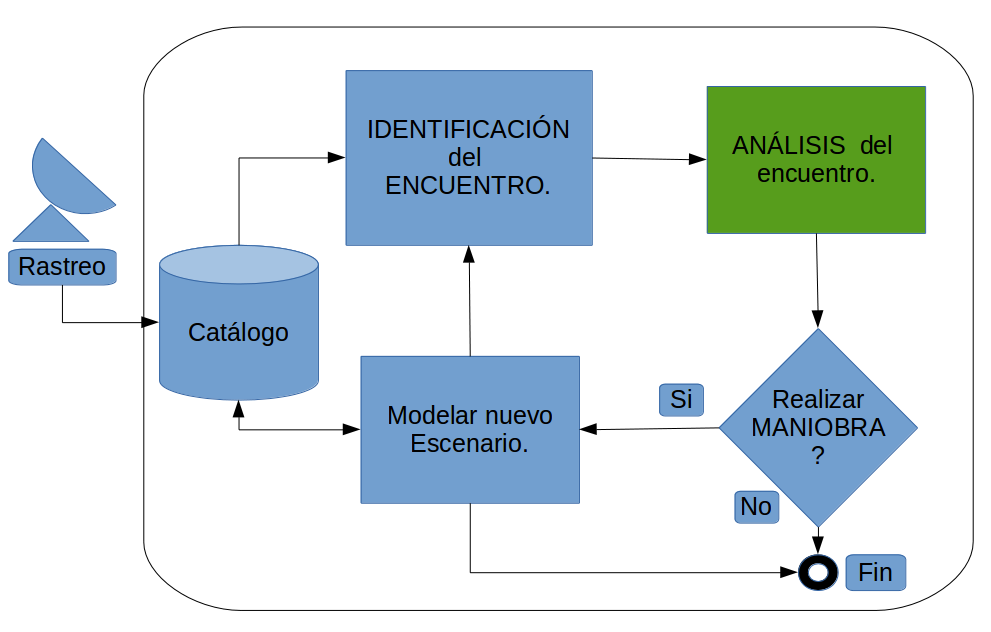
\includegraphics[width=0.6\textwidth]{imagenes/estudiocolision}
  \caption[Estudio de Colisi\'on]{Esquema de alto nivel de los procesos en un estudio completo de riesgos de colisi\'on. (Se indica en color verde, la etapa que se desarrolla en este trabajo.)}
  \label{fig:estudiocolision}
\end{figure}


% CONCEPTO DE MIDDLE MAN.\\
% CONCEPTO DE COLLABORATIVE WORK ENVIRONMENT. (close loop process)

\subsection{Rastreo y cat\'alogos}\label{subsec:redes}

En los catálogos actuales se registran objetos mayores a los 10 cent\'imetros en las regiones LEO monitoreadas con radares, y mayores a 1 metro en las \'orbitas \ac{GEO} observadas con telescopios \'opticos.\\
 
La entidad militar \ac{USSTRATCOM} de los Estados Unidos de Am\'erica (EE.UU) mantiene un catálogo con 18347 objetos conocidos (al 4 de Abril de 2017). Para su construcci\'on y mantenimiento, utiliza la Space Surveillance Network (SSN), que posee m\'as de 20 sensores civiles y militares a lo largo de todo el mundo (Fig.\ref{fig:usnet}).\\

\begin{figure}[!h]
  \centering
  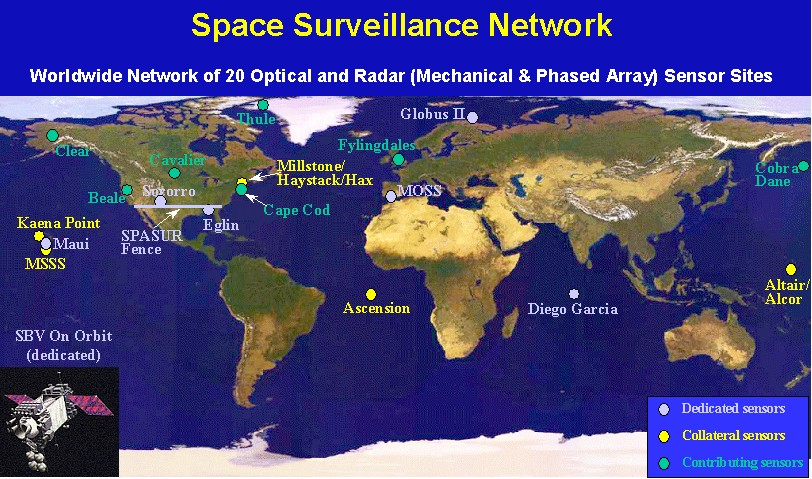
\includegraphics[width=0.7\textwidth]{imagenes/SpSNet}
  \caption[USSTRATCOM - SSN]{US. Strategic Command Space Surveillance Network. Extra\'ido de https://en.wikipedia.org/wiki/United\_States\_Space\_Surveillance\_Network}
  \label{fig:usnet}
\end{figure}

Rusia es la \'unica naci\'on, aparte de los EE.UU, que cuenta con un sistema de rastreo que le proporciona una base de datos de objetos espaciales artificiales significativa y actualizada. A su vez, independiente del gobierno Ruso, el Keldysh Institute of Applied Mathematics (KIAM) promueve la red internacional: International Scientific Optical Network (ISON), que ofrece uno de los programas coordinados de monitoreo de desechos m\'as importante.
La red cuenta con 30 telescopios en el rango de 0.5 a 2.6 metros de di\'ametro, repartidos en 20 observatorios de 8 pa\'ises en todo el mundo.\\

Por su parte, la ESA inici\'o programas de monitoreo hace ya varios a\~nos. En la actualidad predominan las investigaciones realizadas por las agencias espaciales: la Agenzia Spaziale Italiana (ASI) de Italia, el  British National Space Centre (BNSC) de  Inglaterra, el Centre National d'Études Spatiales (CNES) de Francia, y el Deutsche Zentrum fur Luft- und Raumfahrt  (DLR) de Alemania, con el apoyo de la industria, institutos de investigaci\'on y universidades. En los \'ultimos 10 a\~nos han estado trabajando en forma coordinada para implementar un Sistema Europeo de Vigilancia Espacial.
A tal fin cuentan con varios telescopios \'opticos como el Zeiss de 1 metro de Tenerife, el Schimdt y Tarot en Francia, o los sensores PIMS (Passive Imaging Sensors) del Reino Unido, y con importantes radares, como el TIRA (Tracking and Imaging Radar) en Alemania, o los m\'as modernos EISCAT Y EICAT 3D (European Incoherent Scatter Radar) que logran detecciones de objetos del orden de los cent\'imetros a distancias de 800 kil\'ometros.


% \begin{verbatim}
%  Settecerri, T. J et al – “Haystack measurements of the orbital debris environment” – Advances in Space Research 1999.
% Mehrholz, et al – “Beam-park experiments at FGAN” –  AdSpR 2004.
% Igor Molotov, et al – “Faint High Orbital Debris Observations with ISON Optical Network” – 
% Proceedings of the Advanced Moui Optical and Space
% \end{verbatim}



\section{Las regulaciones nacionales e internacionales}

Dado el car\'acter global de esta problem\'atica, distintas naciones y agencias internacionales con gran desarrollo y actividad espacial, se han estado organizado en la b\'usqueda de acuerdos y buenas pr\'acticas. Entre los organismos que coordinan las recomendaciones, se encuentran:\\

\begin{itemize}
\item COPUOS: Committee of the Peacefull Uses of Outer Space, \ac{ONU}
\item IADC: Inter-Agency Space Debris Coordination Committee
\item CCSDS: Consultative Committee for Space Data Systems
\end{itemize}

La NASA fue la primera en adoptar un conjunto de lineamientos para la mitigaci\'on de los desechos espaciales en 1995, que fueron posteriormente incorporados por el gobierno de EE.UU en 1997. \\

En el a\~no 2002 el IADC conformado por diez pa\'ises y la ESA, elabor\'o un nuevo conjunto de lineamientos.
Finalmente en 2007 el subcomit\'e cient\'ifico y tecnol\'ogico del COPUOS aun\'o los esfuerzos y reuni\'o todos los trabajos previos, logrando un consenso en los lineamientos definitivos promulgados por la ONU en 2008, \citep{nasaprogramme}.\\

En lo que respecta a los l\'imites de este trabajo, podemos citar las siguientes Normas, Recomendaciones y Legislaci\'on:\\

\begin{itemize} 
\item Convenio sobre Responsabilidad Internacional por da\~nos causados por objetos espaciales. ONU - (29-03-72)
\item Ley 23.335 (19-08-86) - Arg. Suscribe al Convenio de ONU.
\item Space Debris Mitigation Guidelines - \citep{iadcguide}
\item ISO 24113:2011 {\it{Space Debris mitigation requirements.}}
\item ISO/TR 16158:2013 {\it{Space Systems - Avoiding collision with orbiting objects.}}
\item ISO 19389:2014 {\it{Space data and information transfer Systems.}} Conjunction Data Message: specifies a standard message format for use in exchanging spacecraft conjunction information between originators of Conjunction Assessments (CAs) and satellite owner/operators and other authorized parties.
\item {\it{Guidelines for the long-term sustainability of outer space activities}}. Vienna, 8-17 de Junio de 2016.
\item {\it{CCSDS 508.0-B-1, Conjunction Data Message Recommended Standard}} - \citep{CDM}
\end{itemize}

\section{Antecedentes}
En este contexto, ya existen claros antecedentes que abordan la problem\'atica con sus respectivos soportes inform\'aticos. Ver Tabla \ref{tab:sisal}.
\begin{table}[!h]
\caption[Sistemas de Alerta]{Sistemas de Alertas de distintas Naciones y Agencias}
\begin{tabular}{lp{5cm}p{6cm}}
\hline
Herramienta & Descripci\'on & Proveedor/Agencia\\
\hline
{\bf{CARA}} & {\it{Conjunction Assessment Risk Analysis}} & NASA Robotic Conjunction Assessment Risk Analysis group, en convenio con la empresa a.i. solutions, Inc.\\
\hline
{\bf{SOCRATES}} & {\it{Satellite Orbital Conjuction Reports Assessing Threatening Encounters in Space}}, servicio web v\'ia Celestrack.com & CSSI (Center for Space Standards \& Innovation) de la agencia AGI: Analytical Graphics, Inc.\\
\hline
{\bf{CRASS}} & {\it{Collision Risk Assessment tool}} & Desarrollado por la
empresa GMV, que presta servicios al Centro Europeo de Operaciones
Espaciales (ESOC) - Darmstadt, Alemania, \citep{alarconRodriguez}\\
\hline
{\bf{CAESAR}} & {\it{Conjuction Analysis and Evaluation Service, Alerts and Recommendations}} & Agencia francesa CNES, que utiliza como soporte el Software JAC {\it{Java for Assessment of Conjunctions}}, \citep{laporte}\\
%\hline
%closeap - ant\'on & & ESA\\
\hline
{\bf{CRAMS}} & {\it{Collision Risk Assessment and Mitigation System}} & Canadian Space Agency (CSA), \citep{babiker}.\\
\hline
\end{tabular}
\label{tab:sisal}
\end{table}

\section{La Comisi\'on Nacional de Actividades Espaciales (CONAE)}
De acuerdo con el Plan Nacional Espacial: {\bf{ Argentina en el Espacio 2004-2015}}, las misiones de la CONAE, fundamentalmente pensadas para observaci\'on de la Tierra, ocupan \'orbitas bajas de dise\~no estrat\'egico, (Fig. \ref{fig:Dvsaltura}). Es decir, se ubican en regiones de mucha demanda y en consecuencia se encuentran expuestas a un alto riesgo de colisi\'on.\\

En nuestro pa\'is, compete a la CONAE; quien tiene la facultad de mantener las relaciones con los organismos internacionales, garantizar que se cumplan los distintos convenios y acuerdos a los que Argentina ha adherido, como por ejemplo el {\it{Convenio sobre la Responsabilidad Internacional por da\~nos causados por objetos espaciales}}, suscrito por la Rep\'ublica Argentina el 29 de marzo de 1972 (LEY N 23.335, sancionada: Julio 30 de 1986 - promulgada: Agosto 19 de 1986.1).\\

As\'i mismo, siendo Argentina miembro de la ONU, es la CONAE la representante ante el COPUOS en materia de buenas pr\'acticas para la mitigaci\'on de la generaci\'on de desechos espaciales.\\

Como se indica en la Sec. \ref{subsec:redes}, las \'unicas naciones que cuentan con una red de rastreo con capacidad de detectar, rastrear y catalogar objetos son los EE.UU y Rusia. De manera que la Argentina planifica y ejecuta sus maniobras de riesgo a partir de informaci\'on que le proveen servicios externos.\\

\section{Planteo del Problema}

El desfavorable panorama futuro en materia de colisiones en \'orbita, obliga a los centros de operaciones a incorporar procedimientos y soportes, para la gesti\'on, el an\'alisis y la prevenci\'on de las colisiones.\\

Dependiendo de las distintas capacidades con que cuentan las agencias, estos sistemas incluyen desde: redes o instrumentos espec\'ificos de rastreo propios, cat\'alogos completos de los objetos capaces de ser rastreados, sistemas de detecci\'on anticipada de acercamientos de riesgo, sistemas de an\'alisis de situaciones de riesgo alertadas por agentes externos o contrataci\'on de servicios externos que resuelven la totalidad del an\'alisis incluyendo la sugerencia de las maniobras pertinentes.\\

Argentina no cuenta actualmente con una red de rastreo para generar sus propios cat\'alogos y tampoco se desarroll\'o a\'un un sistema que permita
analizar los cat\'alogos ya existentes de acceso p\'ublico para el estudio de riesgo de colisi\'on de sus misiones.\\

Para cubrir este aspecto, la CONAE contrata un servicio externo de asesoramiento y control para la predicci\'on de los acercamientos de riesgo y la planificaci\'on de las operaciones necesarias. Ofrecer un servicio que lo reemplace, es impensado y escapa por mucho a los alcances de este trabajo.\\

En este trabajo se presenta una herramienta que tiene la capacidad de incorporar alertas de riesgo de colisi\'on; ya sea a trav\'es de un \ac{CDM} o por ingesta manual, mostrar mediante una interfaz gr\'afica amigable esos valores que se ingresaron, hacer un registro ordenado de las distintas situaciones y, en paralelo, calcular con sus propios m\'etodos, los par\'ametros de caracterizaci\'on del riesgo, a fin de evaluar la precisi\'on y las limitaciones del software.\\

La herramienta ARxCODE para el An\'alisis de Riesgo por Colisi\'on con Desechos, que presentamos en esta tesis, consiste en un prototipo de software para ser utilizado por operadores con amplios conocimientos de din\'amica orbital y operaciones.\\

Su capacidad para automatizar la recepci\'on de mensajes de alerta y desglozar el contenido, para presentarlo en forma m\'as amigable, pretende ofrecer una clara visualizaci\'on de la situaci\'on y un mayor conocimiento al operador, para enriquecer el di\'alogo e intercambio de informaci\'on con los organismos y agencias que proveen el servicio y asesoramiento.\\

La facilidad de utilizar la informaci\'on predicha (o recibida), seleccionar la configuraci\'on deseada y realizar un procesamiento propio, se piensa como un planteo preliminar, con versatilidad para ser probado, perfeccionado y ampliado a largo plazo.\\


El mismo oficiar\'a de soporte al operador de din\'amica orbital, quien se encargar\'a de procesar la informaci\'on con las facilidades que ARxCODE provee y generar los reportes necesarios que faciliten el intercambio de informaci\'on y la toma de decisiones, (Fig. \ref{fig:arcodeInterface}). \\ 


\begin{figure}[!h]
\centering
  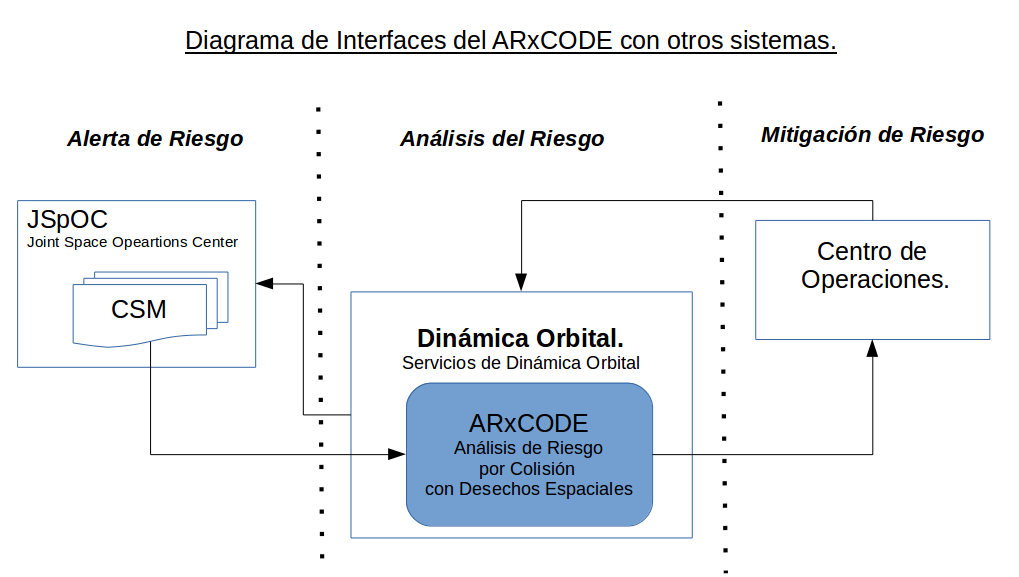
\includegraphics[width=0.7\textwidth]{imagenes/interfasessistemas}
  \caption[Interfaces del ARxCODE]{Esquema de Interfaces entre ARxCODE el orgamismo externo que envia el mensaje de alerta JSpOC, el Departamento de Din\'amica Orbital y el Centro de Control.}
  \label{fig:arcodeInterface}
\end{figure}



\section{Objetivos}

\subsection*{Objetivo principal}
Dise\~nar un procedimiento operativo frente a situaciones de alerta por riesgo de posible
colisi\'on con desechos espaciales y desarrollar un prototipo de software: ARxCODE, que
permita el c\'alculo de los par\'ametros de caracterizaci\'on del riesgo y facilite al analista la
la comprensi\'on y visualizaci\'on de la situaci\'on de riesgo en el di\'alogo con los servicios de alerta externos.\\

\subsection*{Objetivos espec\'ificos}
\begin{itemize}
\item Automatizar la recepci\'on y gesti\'on de los mensajes de alertas (CDM) por posibles
colisiones, que se reciben de organismos internacionales de rastreo.
\item Desarrollar una t\'ecnica que mejore la estimaci\'on de los errores en la posici\'on del desecho espacial.
\item Calcular la \ac{PoC} para caracterizar la situaci\'on de encuentro.
\item Desarrollar un prototipo de software (ARxCODE) para el procesamiento de la informaci\'on, el manejo de las notificaciones, la visualizaci\'on del evento y la generaci\'on de reportes.
\end{itemize}

\section{Estructura del trabajo}

A continuaci\'on de esta introducci\'on, en el cap\'itulo de {\bf{Marco Te\'orico}}; se describen los conceptos te\'oricos que se relacionan a la problem\'atica de las colisiones. Se detallan las distintas maneras en que se calculan las posiciones de los objetos seg\'un sean misiones operativas o desechos espaciales, los modelos de propagaci\'on, los formatos de publicaci\'on de la informaci\'on y los sistemas de referencia que utilizamos en este trabajo. En este cap\'itulo se dedica una secci\'on especial para el tratamiento de los errores en las posiciones y en las propagaciones, donde se describen el m\'etodo de Osweiler, \citep{osweiler} y el m\'etodo de propagaci\'on propuesto. Contin\'ua la secci\'on que contiene la informaci\'on te\'orica referida al c\'alculo de la probabilidad de colisi\'on (m\'etodo de Lei-Chen, \citep{leichen}) y finalmente una secci\'on dedicada al mensaje estandarizado de alerta \ac{CDM}.

En el cap\'itulo 3 de {\bf{Metodolog\'ia de Desarrollo}}, se indican las distintas fases del desarrollo incremental del prototipo de software ARxCODE    y las especificaciones correspondientes al entorno de desarrollo. 

El cap\'itulo 4: {\bf{ARxCODE}}, contiene una descripci\'on detallada del prototipo de software; sus especificaciones, requerimientos, interfaces, casos de uso, arquitectura y flujo. 

En el cap\'itulo de {\bf{Validaciones y Resultados}} se muestran los resultados m\'as significativos que se obtienen al utilizar el ARxCODE, y resultados intermedios que fueron necesarios para la generaci\'on de los productos finales. En cada caso se indica la fuente que se utiliz\'o para validarlos y se presentan valores comparativos en tablas o gr\'aficos. Al final del cap\'itulo se realiza un an\'alisis de los mismos. 

Finalmente el cap\'itulo 6, contiene las {\bf{Conclusiones}} y el trabajo a futuro. 


\endinput